% !TeX program = xetex
% 本报告由 tectonic（XeTeX 引擎）编译：tectonic result/report.tex
% 所有数值均来自生产时归档产物；当前 Git 交付保留汇总、清单和小型证据，
% 但不包含生产数据、模型权重和原始反演分片。可核验范围与缺失项见附录。
\documentclass[UTF8,a4paper,11pt]{ctexart}
\usepackage{geometry}
\geometry{margin=2.5cm}
\usepackage{amsmath,amssymb}
\usepackage{booktabs}
\usepackage{graphicx}
\usepackage{multirow}
\usepackage{array}
\usepackage{caption}
\usepackage{float}
\usepackage{hyperref}
\hypersetup{colorlinks=true, linkcolor=black, citecolor=blue, urlcolor=blue}
\captionsetup{font=small, labelsep=quad}
\emergencystretch=2em

\title{\textbf{面波频散正演代理与反演实验技术报告}\\
\large ——\texttt{swave-forward} 项目：百万样本数据集、四头神经代理、\\
基于代理的 L-BFGS-B、监督反演与灵敏度加权混合反演实验}
\author{}
\date{2026 年 8 月 17 日}

\begin{document}
\maketitle

\begin{abstract}
\noindent 本报告系统总结 \texttt{swave-forward} 项目（纯 Python 瑞利波正演求解器与神经代理）
已完成的全部工作与真实实验结果，覆盖：确定性地质模型生成与百万样本数据集构建、
共享骨干四模态输出神经代理的训练、基于可微代理的 L-BFGS-B 反演实验
（10 万样本全量单起点群体实验与 400 样本 \(\times\) 100 起点的深度多起点实验，
各含无噪声与 1\% 高斯噪声两种观测情景）、三种子监督直接反演的正式 GPU 训练与
独立测试，以及把监督预测按逐层频散灵敏度加权后嵌入 L-BFGS-B 的混合反演生产实验。
所有已报告指标均直接取自归档产物，未使用
其他划分的结果补值。

主要结果：（1）正演求解器完成 100 万样本生产数据集，零恢复、零拒绝；逐样本审计
确认四类合成模型规则全部满足，样本 ID、Vs 和完整记录均无精确重复或跨折重复；
（2）正演代理在独立测试集的总体掩码 MAE 为 \(1.80\times10^{-4}\) km/s，验证集
MAE 为 \(1.82\times10^{-4}\) km/s；（3）旧窄边界反演在 90--99 保留折的 clean 与
1\% 高斯噪声情景各运行 10 万行，全部 100\% 收敛；代理频散重构 MAE 仅 0.0064 km/s，
但 clean 的 Vs 恢复 MAE 高达 0.304 km/s（平均相对误差 20.8\%），深部层（1.6 km 以下）
误差达 0.7 km/s 量级且呈系统性
负偏差；1\% 观测噪声对恢复精度几乎无影响（成对差 \(+5.6\times10^{-4}\) km/s）；
（4）四族等量的 400 样本深度多起点实验绝对 Vs MAE 为 0.271 km/s，P10--P90 经验区间
覆盖率仅 49.7\%（名义 80\%），深部层覆盖率趋近于零；因其人口权重与 10 万样本全量实验
不同，二者总体 MAE 差不能归因于多起点；（5）三种子监督集成在 85--89 正式测试折的
Vs MAE 为 0.02629 km/s，在 90--99 同样本比较折为 0.02633 km/s，比当前 L-BFGS-B clean
的 0.30444 km/s 低 91.35\%；该比较已由原始反演分片重建的精确样本身份通过机器校验；
（6）混合反演在验证候选中选择 \(\lambda_p=1.0\)，在
90--99 折 clean/noise\_1pct 下的 Vs MAE 为 0.02739/0.05491 km/s，相比无学习先验的
全局边界控制组降低 89.34\%/78.64\%；clean 下平均迭代数降低 28.89\%。但最优系数位于候选
上边界，且 1\% 高斯噪声使学习型方法误差约翻倍。结果表明学习型合成先验能显著减少当前
优化协议的深部系统偏差，但不能替代对实测地质、随机缺失或其他分布外扰动的验证。
\end{abstract}

\tableofcontents
\newpage

\section{引言}
近地表瑞利波频散反演是浅层横波速度结构成像的核心手段。含低速夹层（low-velocity
layer, LVL）的层状半空间中，频散曲线存在密集的``模式接吻''（mode-kissing）根，
对正演求根的稳健性与反演的非唯一性处理都提出了挑战。本项目以 Pan 与 Chen 的
mode-kissing 参考实现\cite{pan-mode-kissing}和 Pan 等人的 QEDispInv 反演框架
\cite{pan-qedispinv}
为算法来源，以纯 Python（NumPy/Numba/SciPy/PyTorch）实现了完整管线：
确定性模型生成 \(\to\) 物理正演 \(\to\) HDF5 数据集 \(\to\) 神经代理训练
\(\to\) 基于代理的反演 \(\to\) 自动报告。两个参考仓库仅提供算法与测试夹具，不作为
运行时依赖。

固定的生产问题定义为：20 个 Vs 值（0.30--2.60 km/s），19 个 0.1 km 有限层加
1.9 km 起算的半空间；频率 0.5--60.0 Hz、步长 0.5 Hz（120 点）；瑞利波 0--3 阶
模式；模型族包括正常（normal）、低速（LVL）、高速（HVL）与高低耦合（coupled）四类。
全文深度单位为 km，速度为 km/s，频率为 Hz。

本文余下结构：第 \ref{sec:method} 节给出方法，第 \ref{sec:data} 节为数据集构建结果，
第 \ref{sec:surrogate} 节为代理训练与精度，第 \ref{sec:inversion} 节为反演实验主结果，
第 \ref{sec:supervised} 节给出监督反演训练结果与同样本比较，第 \ref{sec:hybrid} 节给出
灵敏度加权学习先验混合反演的生产结果，第 \ref{sec:discussion} 节讨论未达预期的
结果及其影响，第 \ref{sec:conclusion} 节总结。附录 \ref{app:repro} 列出可复现性与完整性证据。

\section{方法}\label{sec:method}

\subsection{正演求解器}
正演核心（\texttt{src/swave/secular.py}, \texttt{solver.py}）传播未归一化的
瑞利波 Dunkin \(\delta\) 矩阵，用 TOMS 748 在符号变号区间内求根；标量热路径由
Numba JIT 缓存。初始采样沿用参考实现的模态计数估计。为处理模式接吻，实现了两种
恢复策略：\texttt{degraded}（浅化退化模型的根补充完整模型）与 \texttt{quadratic}
（默认；二次极值在同号区间内补采样，可能含成对靠近根）。二次粗扫描在 4 个目标根加
2 个偏置根后停止，与参考算法的有界搜索一致。高阶模式的合法前导缺口保持掩码；
内部缺口或数值失败仅允许一次有界细化，随后触发确定性模型重生成——代码从不以零值
或插值静默填充缺失物理目标。物理参数：\(\epsilon=0.5\)，\texttt{nfine}=2，
二次迭代 3 次，根容差 \(10^{-8}\)，去重容差 \(10^{-7}\)。

求解器正确性由测试夹具（\texttt{tests/test\_reference.py} 及
\texttt{tests/fixtures}）对照参考实现的可溯源输出验证。

\subsection{确定性地质模型生成与数据集格式}
模型生成（\texttt{geology.py}）由 \((\text{全局种子},\text{样本ID},\text{重试计数})\)
完全确定。背景模型表层 Vs 均匀采样，半空间 Vs 不低于表层 \(+0.6\) km/s；
异常置于第 3--12 层：低速族为连续 1--3 层负异常，高速族为连续 1--2 层正异常，
耦合族为 1 层高速异常后紧邻连续 2--3 层低速异常；异常相对背景的对比度均在
8\%--35\% 之间。正常族不含异常。四类模型目标比例：正常 0.25、低速 0.15、
高速 0.10、耦合 0.50。Vp 与密度由
Brocher (2005) 经验关系（\texttt{empirical\_method = brocher05}）从 Vs 换算。

数据集（\texttt{configs/dataset.toml}）：100 万接受样本，100 个分片
（每片 10{,}000），全局种子 20260727，最大重试 8 次。每个
\texttt{shard-NNNNN.h5} 含样本 ID、模型族、20 层 Vs/Vp/密度、
\((4\times120)\) 相速度目标（缺失单元为 NaN）、有效掩码、质量标志与重试计数；
gzip 压缩、临时路径写入、完整关闭后原子重命名。\texttt{manifest.json} 记录配置哈希、
包版本、逐分片 SHA-256、各族接受/拒绝计数与恢复计数；恢复训练或评估前逐分片重新
校验全部数据形状、dtype、样本 ID 摘要、物性不变量、曲线掩码与文件校验和。

\subsection{数据划分策略}
划分仅由 \(\text{样本ID} \bmod 100\) 决定，跨分片稳定：0--79 训练（80\%），
80--84 验证（5\%），85--89 测试（5\%），90--99 反演保留（10\%），策略标识
\texttt{mod100-v2-80-5-5-10}。训练折只用于拟合与归一化统计，验证折只用于检查点选择，
测试折用于正演代理和监督反演的最终测试，反演保留折用于第 \ref{sec:inversion} 节的
优化反演。监督模型全部定型后可对反演保留折做一次只读推理，以便与优化反演在相同
样本上比较；该结果不参与训练、早停、超参数或种子选择。

\subsection{四头神经代理}\label{sec:net}
代理网络（\texttt{network.py} 中 \texttt{FourHeadForwardModel}）将 20 个 Vs 映射为
4 条独立的 120 频率模态曲线：输入层（20\(\to\)256, GELU），4 个残差 MLP 块
（256\(\to\)512\(\to\)256，GELU，LayerNorm，宽度 256），4 个独立输出头
（256\(\to\)256\(\to\)120）。全模型共 1{,}445{,}600 参数（由实现实例化统计）。
损失为各非空模态独立平均的掩码 Smooth-L1 再取模态平均；归一化统计仅用训练划分的
有效单元计算。

生产训练配置（\texttt{configs/training-48g.toml}）：批 8192，300 轮，AdamW
（lr \(10^{-3}\)，weight decay \(10^{-4}\)），CosineAnnealingLR（\(T_{\max}=300\)），
64 个数据加载进程，CUDA 设备（48 GB 显存档位配置，于外部主机执行），种子 20260727，
断点可恢复（\texttt{last.pt}/\texttt{best.pt}/\texttt{history.json}）。

\subsection{基于代理的 L-BFGS-B 反演}\label{sec:inv-method}
反演（\texttt{inversion.py}, \texttt{inversion\_runner.py}）仅基于观测数据进行：
源数据集真值不参与初始化、边界、目标、梯度与优化，仅由报告器在全部结果身份与分片
校验通过后才联接真值。每个样本在两种情景下分别运行并独立报告：\texttt{clean}
（原始曲线）与 \texttt{noise\_1pct}（仅对有效模态单元加 1\% 相对高斯噪声）。

\paragraph{参考模型与边界} 参考模型仅由基阶有效观测构造：深度近似
\(d \approx v_{\text{ph}}/(3f)\)，层速度取 \(1.1\,v_{\text{ph}}\)，经两次
\([0.25,0.5,0.25]\) 平滑后插值到 20 层网格并截断到 \([0.3,2.6]\) km/s。
逐层搜索边界为参考值 \(\pm 0.35\) km/s（\texttt{vs\_width = 0.7}）与全局边界的交。

\paragraph{目标函数} 有界 L-BFGS-B（\texttt{max\_iterations=100}，相对容差
\(10^{-5}\)）最小化
\begin{equation}
J(\mathbf{v}) = \sum_{m=0}^{3} w_m \cdot \mathrm{mean}_{\text{有效单元}}
\big(F_m(\mathbf{v}) - d_m\big)^2
+ \frac{\lambda}{20}\,\big\| R\,(\mathbf{v}-\mathbf{v}_{\text{ref}})\big\|^2 ,
\end{equation}
其中 \(F\) 为可微代理（float64，autograd 同遍给出值与梯度），模态权重
\(\mathbf{w}=(4,1,1,1)\)，\(\lambda=0.01\)，\(R\) 为 QEDispInv 式自适应一阶差分
矩阵（\(\texttt{regularization\_type=adaptive}\)：权重
\(\alpha/(\alpha+|\Delta v_i|)\)，\(\alpha=0.1\max|\Delta v|\)）。

\paragraph{全量单起点实验（full）} 反演保留划分全部 100{,}000 个样本，每样本每情景
从参考模型做 1 次优化，共 200{,}000 行。

\paragraph{深度多起点实验（deep）} 按族分层抽取 400 样本（每族 100），每样本每情景
100 个起点（参考模型加 99 个确定性平滑高斯扰动，截断于边界内），共 80{,}000 次优化。
目标值按含零 IQR 情形的闭区间 1.5-IQR 栅栏剔除离群起点；样本成功要求至少 20 个有效解
（\texttt{minimum\_valid\_solutions}）。恢复模型取内点起点的逐层中位数，P10/P90 给出
经验区间；并用物理 Dunkin 求解器对恢复模型独立重校验（其成功/状态/失败码与反演集成的
相应字段相互独立）。深度工作切分为确定性作业（每作业 10 样本、至多 1000 次起点），
80 个作业按模分配支持多任务并行与断点恢复。

\subsection{监督直接反演}
监督基线由 \texttt{supervised\_inversion.py} 完整实现。输入为 4 个模态去掉 0.5 Hz
频点后的展平频散向量（476 维 \(=4\times119\)），输出为 20 层 Vs。网络采用宽度
1024 的 GELU 输入干、4 个 Pre-LN 残差块、最终 LayerNorm 与线性输出头，共
8{,}915{,}988 个参数。无效频点填充值、输入均值/标准差和 Vs 均值/标准差全部只由
0--79 训练折流式统计。训练采用 Huber 损失、AdamW（lr \(10^{-3}\)，weight decay
\(10^{-4}\)）、CosineAnnealingLR、批量 8192；种子 0、1、2 各至多 150 轮，且只按
80--84 验证折的物理 Vs MAE 选择检查点和早停。三个最佳检查点等权集成后才读取
85--89 测试折，并额外对 90--99 反演保留折做同样本只读比较。检查点绑定数据集配置
哈希、清单 SHA-256、有序三种子集合、训练样本摘要、归一化数组、网络与训练配置，
恢复时任何不一致都会报错。数据加载按分片内属于目标折的连续区间成批读取，再以
种子与轮次派生的确定性顺序打乱逻辑批，避免对 gzip HDF5 做逐样本随机解压；轮次随机性
同样由种子与轮次确定性派生。每轮先原子发布最佳权重和历史，最后以
\texttt{last.pt} 作为轮次提交标记，因此中断恢复与连续训练轨迹一致，已满足耐心阈值
的种子再次运行也不会额外训练。

\subsection{灵敏度加权学习先验的混合反演}\label{sec:hybrid-method}
为同时利用监督反演从 80 万训练标签中学习到的统计先验和当前样本的频散物理约束，
新增混合反演（\texttt{hybrid\_inversion.py}, \texttt{hybrid\_runner.py}）。对当前
观测按第 2.6 节完全相同的训练折统计做填充和归一化，三个最佳监督检查点分别预测
20 层 Vs，等权平均得到学习先验
\begin{equation}
\mathbf v^{\mathrm{sup}}=\frac{1}{3}\sum_{k=1}^{3}
\mathbf v^{\mathrm{sup},k}.
\end{equation}
该向量只作为软正则中心，不作为 L-BFGS-B 初值、硬边界或停止条件。

\paragraph{逐层灵敏度与权重}
在 \(\mathbf v^{\mathrm{sup}}\) 处对 float64 正演代理计算完整雅可比。第 \(i\) 层的
无量纲平均绝对灵敏度定义为
\begin{equation}
s_i=\frac{\displaystyle\sum_{m,f}I_{m,f}w_m
\left|\frac{v_i^{\mathrm{sup}}}{F_{m,f}}
\frac{\partial F_{m,f}}{\partial v_i}\right|}
{\displaystyle\sum_{m,f}I_{m,f}w_m},
\end{equation}
其中 \(I_{m,f}\) 为当前样本有效掩码，模态权重仍为 \((4,1,1,1)\)。只统计有限、
有效且预测相速度高于数值安全阈值的单元；无有效灵敏度或非有限雅可比直接记为失败，
不以常数静默替代。学习先验逐层权重取逆灵敏度：
\begin{equation}
r_i=\frac{1}{s_i+\epsilon_s},\qquad
\omega_i=\operatorname{clip}(c r_i,0.25,4.0),\qquad
\frac{1}{20}\sum_{i=1}^{20}\omega_i=1.
\end{equation}
\(\epsilon_s\) 为样本平均灵敏度的固定小比例，缩放系数 \(c\) 由单调二分求解。
因此低灵敏度层获得更强先验约束，高灵敏度层保留更多由当前频散修正监督预测的自由度。
灵敏度和权重在每个样本优化前只计算一次，迭代中保持不变。

\paragraph{混合目标与控制组}
混合 L-BFGS-B 最小化
\begin{equation}
J_{\mathrm{hybrid}}(\mathbf v)=J_{\mathrm{disp}}(\mathbf v)
+\frac{\lambda_s}{20}\|R(\mathbf v-\mathbf v_{\mathrm{ref}})\|_2^2
+\frac{\lambda_p}{20}\sum_{i=1}^{20}
\omega_i(v_i-v_i^{\mathrm{sup}})^2,
\end{equation}
其中 \(\lambda_s=0.01\)，\(R\) 与原 L-BFGS-B 相同；\(\lambda_p\) 是唯一新增的
全局强度。优化仍从观测构造的 \(\mathbf v_{\mathrm{ref}}\) 开始，但使用全局物理边界
\([0.3,2.6]\) km/s。为分离``放宽旧窄边界''和``学习先验''的贡献，对每个样本另以
完全相同的初值、全局边界和优化器运行 \(\lambda_p=0\) 控制组。\(\lambda_p\) 只在
80--84 验证折的四族等量样本上按 clean 与 noise\_1pct 综合 Vs MAE 选择；并列时取
更小值。85--89 测试折与 90--99 反演保留折不参与调参。

\section{数据集构建结果}\label{sec:data}
生产数据集 \texttt{data/production}（创建于 2026-08-04）完整完成：
100/100 分片校验通过，接受 1{,}000{,}000 模型，\textbf{恢复 0 次、拒绝 0 次}。
各族接受数：耦合 500{,}418、正常 250{,}028、低速 149{,}812、高速 99{,}742，
与目标比例（0.50/0.25/0.15/0.10）一致。

\paragraph{地质规则与物性审计}
对 100 万条记录执行流式重建审计
（\path{docs/final-report/evidence/dataset-audit.json}）：由
全局种子、样本 ID 与重试计数重新生成的模型与归档 Vs、Vp、密度逐条一致，模型族规则
违规为 0。低速族的 1、2、3 层异常分别为 50{,}043、49{,}648、50{,}121 个；高速族的
1、2 层异常为 49{,}776、49{,}966 个；耦合族总异常层数为 3、4 层的样本分别为
250{,}193、250{,}225 个。异常只出现在层索引 2--11（深度 0.2--1.1 km），实测对比度
范围为低速 8.0008\%--34.9998\%、高速 8.0001\%--34.9999\%、耦合
8.0000\%--34.9999\%。正常背景随深度不减，所有速度与 Brocher 派生物性均通过配置
范围检查。

这些规则符合本实验所需的基本一维地质先验：背景速度总体随压实深度增加，局部低速层
可表征松散、含水或软弱夹层，高速层可表征较致密或胶结层，耦合模型则表达硬层覆盖软层
的局部速度反转；异常连续、幅度有界且不落在半空间之外。不过，这只是参数化合成模型的
内部物理合理性，未结合具体场地的钻孔、测井或构造资料，不能等同于真实地质验证。

\paragraph{唯一性与跨折查重}
样本 ID 共 1{,}000{,}000 个，全部唯一、连续，四个划分计数严格为
800{,}000/50{,}000/50{,}000/100{,}000。以 float32 原始字节为准分别对 20 维 Vs
和完整物理记录计算 SHA-256，并对摘要候选做原始字节复核：两种口径的重复组、重复行和
跨折重复组均为 0。因此没有发现精确数据重复或由重复导致的跨折泄漏。该结论针对逐位
相同记录；物理上接近但数值不同的样本不被误判为重复。

README 记录的单机基准（2026-07-27，相同物理与地质配置；192 逻辑 CPU 主机）：
单 worker 完整 100 模型分片约 210 s（0.476 模型/s）；10 模型样本的平均长期方程
求值 13{,}057 次/模型；压缩后约 1{,}359 字节/模型。据此的规划性外推（假设分片级
理想线性扩展）：单 worker 全量约 24.3 天，100 并发分片约 5.8 小时，压缩存储约
1.36 GB。该外推为规划估计而非完成保证。

\section{正演代理训练与精度}\label{sec:surrogate}
生产运行 \texttt{runs/production-48g} 完整训练 300 轮（\texttt{history.json} 记录
300 条）。验证集掩码 MAE（km/s，物理单位）轨迹：第 0 轮 \(7.96\times10^{-3}\)；
第 10 轮 \(2.18\times10^{-3}\)；第 50 轮 \(1.13\times10^{-3}\)；第 100 轮回升至
\(2.83\times10^{-3}\)（非单调波动）；第 200 轮 \(4.26\times10^{-4}\)；末轮（299）
\(1.82\times10^{-4}\)，为全程最优，\texttt{best.pt} 即末轮权重。最终训练损失
\(2.68\times10^{-6}\)，学习率余弦退火至 \(2.7\times10^{-8}\)。

\paragraph{独立测试集正演评估}
使用当前检查点 \texttt{runs/}\allowbreak\texttt{production-48g/}\allowbreak
\texttt{best.pt} 对样本 ID 余数 85--89 的
50{,}000 个测试样本完成正演评估（表 \ref{tab:forward-test}；JSON 证据归档于
\path{docs/final-report/evidence/forward-test-evaluation.json}）。
四模态合并的有效单元数为
23{,}940{,}013，总体掩码 MAE 为 \(1.80\times10^{-4}\) km/s，RMSE 为
\(4.19\times10^{-4}\) km/s，与验证 MAE \(1.82\times10^{-4}\) km/s 一致，未见明显
泛化落差。误差随模态阶数升高而增大，M3 的 MAE 约为 M0 的 3.27 倍；因此后续反演
仍需保留分模态诊断，不能只依赖总体平均值。

\begin{table}[H]
\centering
\caption{当前四折协议下 85--89 测试折的正演代理精度（50{,}000 个样本）}
\label{tab:forward-test}
\begin{tabular}{lcccc}
\toprule
模式 & MAE (km/s) & RMSE (km/s) & P95 绝对误差 (km/s) & 有效单元数 \\
\midrule
M0 & \(8.89\times10^{-5}\) & \(1.79\times10^{-4}\) & \(2.68\times10^{-4}\) & 6{,}000{,}000 \\
M1 & \(1.36\times10^{-4}\) & \(2.83\times10^{-4}\) & \(4.38\times10^{-4}\) & 5{,}999{,}971 \\
M2 & \(2.05\times10^{-4}\) & \(4.43\times10^{-4}\) & \(6.97\times10^{-4}\) & 5{,}992{,}445 \\
M3 & \(2.90\times10^{-4}\) & \(6.30\times10^{-4}\) & \(1.07\times10^{-3}\) & 5{,}947{,}597 \\
\bottomrule
\end{tabular}
\end{table}

\section{反演实验}\label{sec:inversion}
全部结果取自 \texttt{results/inversion-report/summary.json}（结果模式 v3；报告器在
逐行身份、分片校验和与配置绑定全部验证后才联接真值）。结果身份绑定：数据集清单
SHA-256 \texttt{ceecda31\ldots}、检查点 SHA-256 \texttt{b1a6fc08\ldots}、
数据集配置哈希 \texttt{39cffcbc\ldots}、反演配置哈希 \texttt{d83ad822\ldots}、
软件源码摘要 \texttt{06f66599\ldots}、划分策略 \texttt{mod100-v2-80-5-5-10}。
全量与深度两个范围独立报告，图表从不混合单起点群体行与多起点不确定性行。

\subsection{全量单起点群体实验（100{,}000 样本，200{,}000 行）}
\textbf{收敛性}：200{,}000 行全部成功（状态码 0，成功率 100\%）。平均迭代 22.6 次
（中位 22，P95 38，最大 81），平均函数求值 27.4 次；初始目标均值 0.0417 降至
最终 0.0042（图 \ref{fig:opt-diag}）。

\begin{figure}[H]
\centering
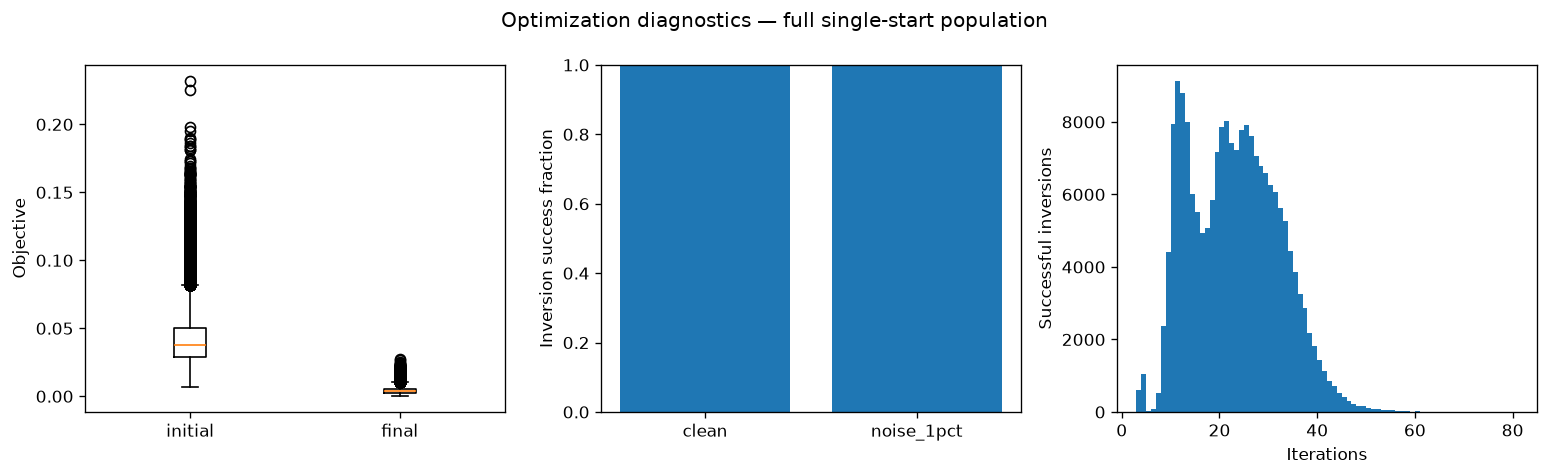
\includegraphics[width=\textwidth]{figures/optimization-diagnostics.png}
\caption{全量单起点群体优化诊断（\texttt{results/inversion-report/optimization-diagnostics.png}）：
初始/最终目标分布、两情景 100\% 成功率、迭代次数直方图。}
\label{fig:opt-diag}
\end{figure}

\textbf{频散重构（代理口径）}：恢复模型经代理预测的曲线相对观测的总体 MAE 为
0.00642 km/s（RMSE 0.0315，P95 0.0172，比较单元 95{,}760{,}266 个，无缺失）；
分模式 M0/M1/M2/M3 的 MAE 分别为 0.00284/0.00438/0.00920/0.00928 km/s。
按情景：clean 0.00503，noise\_1pct 0.00780 km/s。

\textbf{Vs 恢复（主要精度指标）}：表 \ref{tab:full-vs}。总体 Vs MAE 0.3047 km/s、
RMSE 0.4257 km/s、平均相对误差 20.82\%、P95 绝对误差 0.899 km/s。噪声的影响极小：
成对（同一样本两情景均成功）差仅 \(+5.6\times10^{-4}\) km/s（相对误差 \(+0.043\)
个百分点），说明恢复误差由结构性因素主导而非观测噪声。

\begin{table}[H]
\centering
\caption{全量单起点实验 Vs 恢复指标（按情景与模型族；行数为情景\(\times\)样本。
总体行另含 RMSE 0.4257 km/s）}
\label{tab:full-vs}
\small
\begin{tabular}{llcccc}
\toprule
情景 & 族 & 行数 & MAE (km/s) & 平均相对误差 & P95 (km/s) \\
\midrule
\multirow{4}{*}{clean}
 & normal        & 25{,}056 & 0.2694 & 17.79\% & 0.8447 \\
 & high\_velocity & 10{,}074 & 0.2639 & 17.40\% & 0.8161 \\
 & low\_velocity  & 14{,}791 & 0.3223 & 22.11\% & 0.9460 \\
 & coupled       & 50{,}079 & 0.3249 & 22.61\% & 0.9213 \\
\midrule
\multirow{4}{*}{noise\_1pct}
 & normal        & 25{,}056 & 0.2703 & 17.86\% & 0.8461 \\
 & high\_velocity & 10{,}074 & 0.2648 & 17.44\% & 0.8182 \\
 & low\_velocity  & 14{,}791 & 0.3225 & 22.12\% & 0.9473 \\
 & coupled       & 50{,}079 & 0.3253 & 22.64\% & 0.9224 \\
\midrule
\multicolumn{2}{l}{总体（两情景合并）} & 200{,}000 & 0.3047 & 20.82\% & 0.8995 \\
\bottomrule
\end{tabular}
\end{table}

正常与高速族恢复显著优于低速与耦合族（约 17\% 对 22\% 相对误差；
图 \ref{fig:vs-kind}）。误差沿深度迅速增长（图 \ref{fig:vs-depth}）：逐层 MAE 由
第 0 层的 0.003 km/s 增至 1.7 km 深度处的 0.772 km/s；偏差自约 1.1 km 起转为显著
负值（1.7 km 处 \(-0.772\) km/s），即深部速度被系统性低估。该形态与逐层搜索边界
直接相关：参考模型由基阶观测按 \(v_{\text{ph}}/(3f)\) 深度经验式构造，深部约束弱，
而 \(\pm0.35\) km/s 的边界又禁止恢复模型远离参考模型，真实模型的高速半空间
（最高 2.6 km/s）落在边界之外时即产生截断型负偏差。

\begin{figure}[H]
\centering
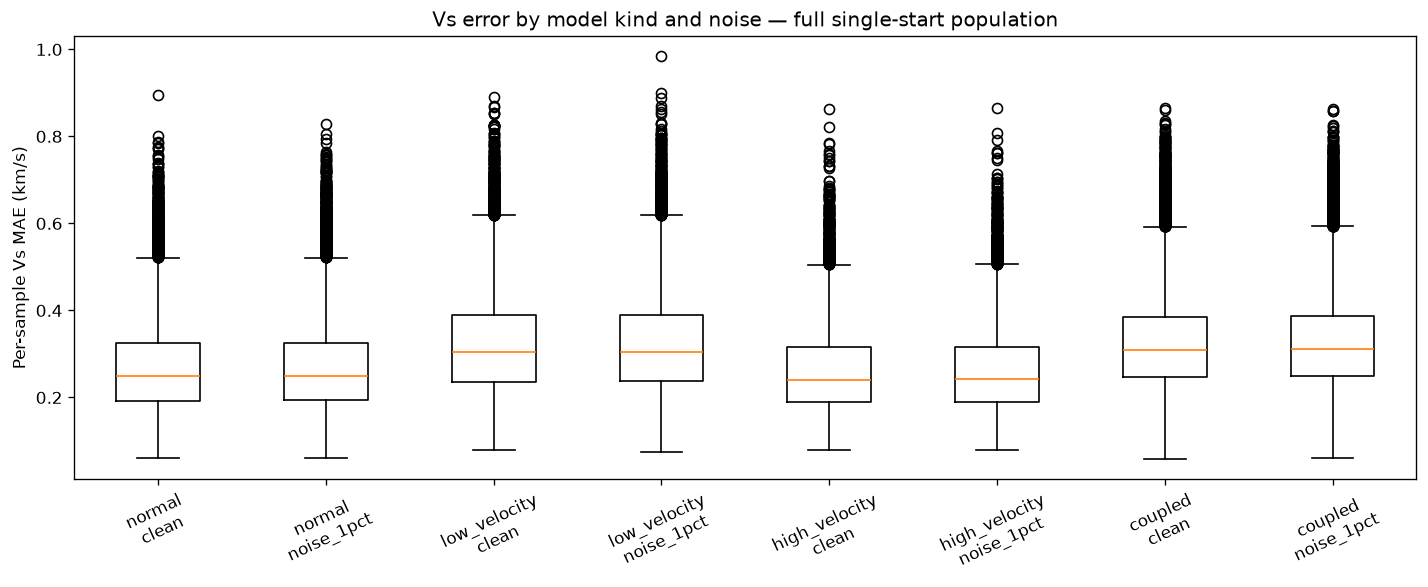
\includegraphics[width=0.95\textwidth]{figures/vs-error-by-kind-and-noise.png}
\caption{全量群体按模型族与噪声情景的单样本 Vs MAE 箱线图
（\texttt{vs-error-by-kind-and-noise.png}）。}
\label{fig:vs-kind}
\end{figure}

\begin{figure}[H]
\centering
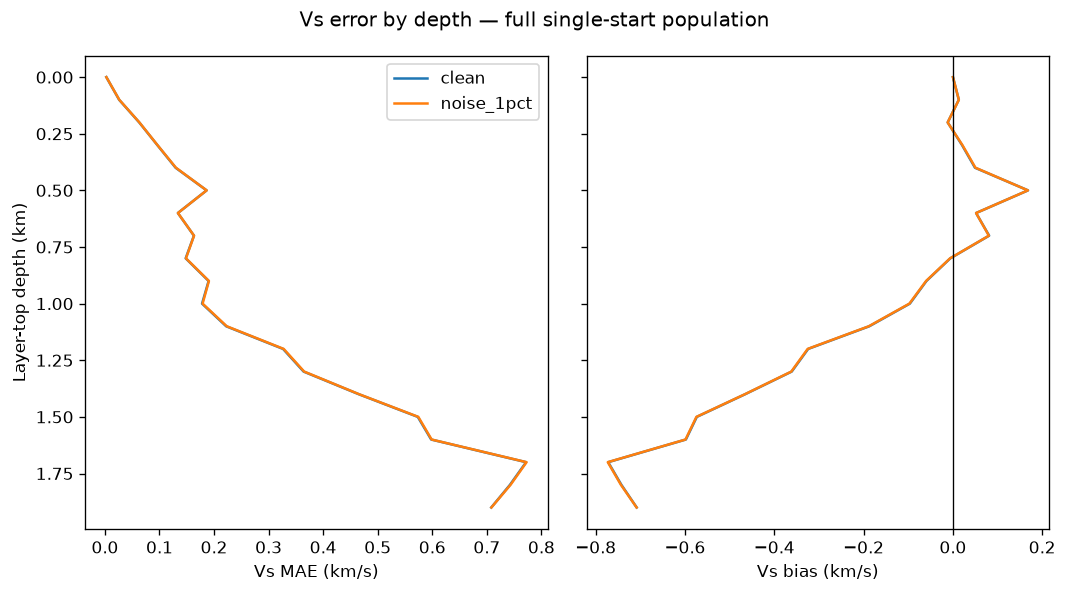
\includegraphics[width=0.95\textwidth]{figures/vs-error-by-depth.png}
\caption{全量群体逐层 Vs MAE 与偏差（\texttt{vs-error-by-depth.png}）。两情景曲线
几乎重合；深部 MAE 接近 0.8 km/s 且偏差达 \(-0.8\) km/s 量级。}
\label{fig:vs-depth}
\end{figure}

\subsection{深度多起点实验（400 样本 \(\times\) 100 起点，800 行）}
\textbf{起点诊断}：80{,}000 次起点全部收敛（100\%）；IQR 栅栏剔除 5{,}300 次
（占成功起点 6.625\%），保留内点 74{,}700 次；单样本被剔起点均值 6.6（最大 23）。
逐样本合计迭代均值 2{,}661 次（单次起点均值 26.6 次、求值 33.3 次）。
800 行全部满足``\(\geq20\) 个有效解''的成功判据。

\textbf{Vs 恢复}：在四族各 100 个模型的等量分层子集上，总体 MAE 0.2713 km/s、
RMSE 0.3906、相对误差 18.32\%、P95 0.848
（clean 0.2710，noise\_1pct 0.2715；成对差 \(+4.8\times10^{-4}\) km/s）。
分族（clean / noise\_1pct）：正常 0.2441 / 0.2458，高速 0.2418 / 0.2407，
低速 0.3128 / 0.3141，耦合 0.2855 / 0.2856 km/s。全量单起点实验使用 10 万模型的
自然族比例，而本实验使用四族等量的 400 模型，样本 ID 与人口权重均不相同；因此不能把
0.3047 与 0.2713 km/s 的差值解释为多起点增益。量化该增益需要在这 400 个相同样本上
另算单起点对照，当前归档汇总不提供这一比较。

\textbf{物理重校验}：800 行的 Dunkin 物理重算全部成功（100\%），物理频散重构
总体 MAE 0.01156 km/s（RMSE 0.0276，P95 0.0637，缺失率 0.27\%），分模式
M0--M3 为 0.0108、0.0104、0.0118、0.0132 km/s；clean 0.0102，
noise\_1pct 0.0130。
值得注意的是，同一恢复模型相对观测的代理残差（总体 0.0155 km/s）大于物理重算残差
（0.0116 km/s），说明拟合优度会随评估算子改变。但物理重算存在 0.27\% 缺失单元，且
当前汇总没有在共同有效单元上直接计算
\(\mathrm{MAE}[F_{\mathrm{proxy}}(\hat{\mathbf v}),
F_{\mathrm{physical}}(\hat{\mathbf v})]\)。因此这两个观测残差不能量化代理在恢复模型上的
外推误差，更不能据此断言代理误差已经超过物理拟合残差；它们只说明保留物理重校验是必要的。

\textbf{不确定性区间（未达预期）}：内点起点 P10--P90 区间的总体覆盖率仅
\textbf{49.7\%}（名义 80\%），平均区间宽 0.295 km/s。逐层覆盖率从浅层的
0.95--0.98 单调退化至深部：1.2 km 以下低于 50\%，1.4--1.9 km 各层覆盖率分别为
0.049、0.021、0.003、0、0、0——深部区间完全不含真值。欠覆盖与第
\ref{sec:inversion}.1 节的系统性负偏差同源：所有起点共享同一有界搜索盒，
当真实深部速度位于盒外时，区间再宽也无法覆盖。

\subsection{代表性样本}
图 \ref{fig:rep-lvl} 与图 \ref{fig:rep-coupled} 分别展示低速族（clean）与耦合族
（noise\_1pct）的代表性深度实验样本（报告器选取规则：各族成功深样本中的最小
样本 ID）。两图共同呈现了本研究的核心现象：
右四幅子图中恢复模型的代理与物理频散曲线与观测几乎重合，而左幅 Vs 剖面中，
中位数恢复模型明显更平滑、深部幅度远低于真值，P10--P90 带在深部亦未能包住真值。
频散拟合优度不能作为 Vs 恢复质量的充分判据。

\begin{figure}[H]
\centering
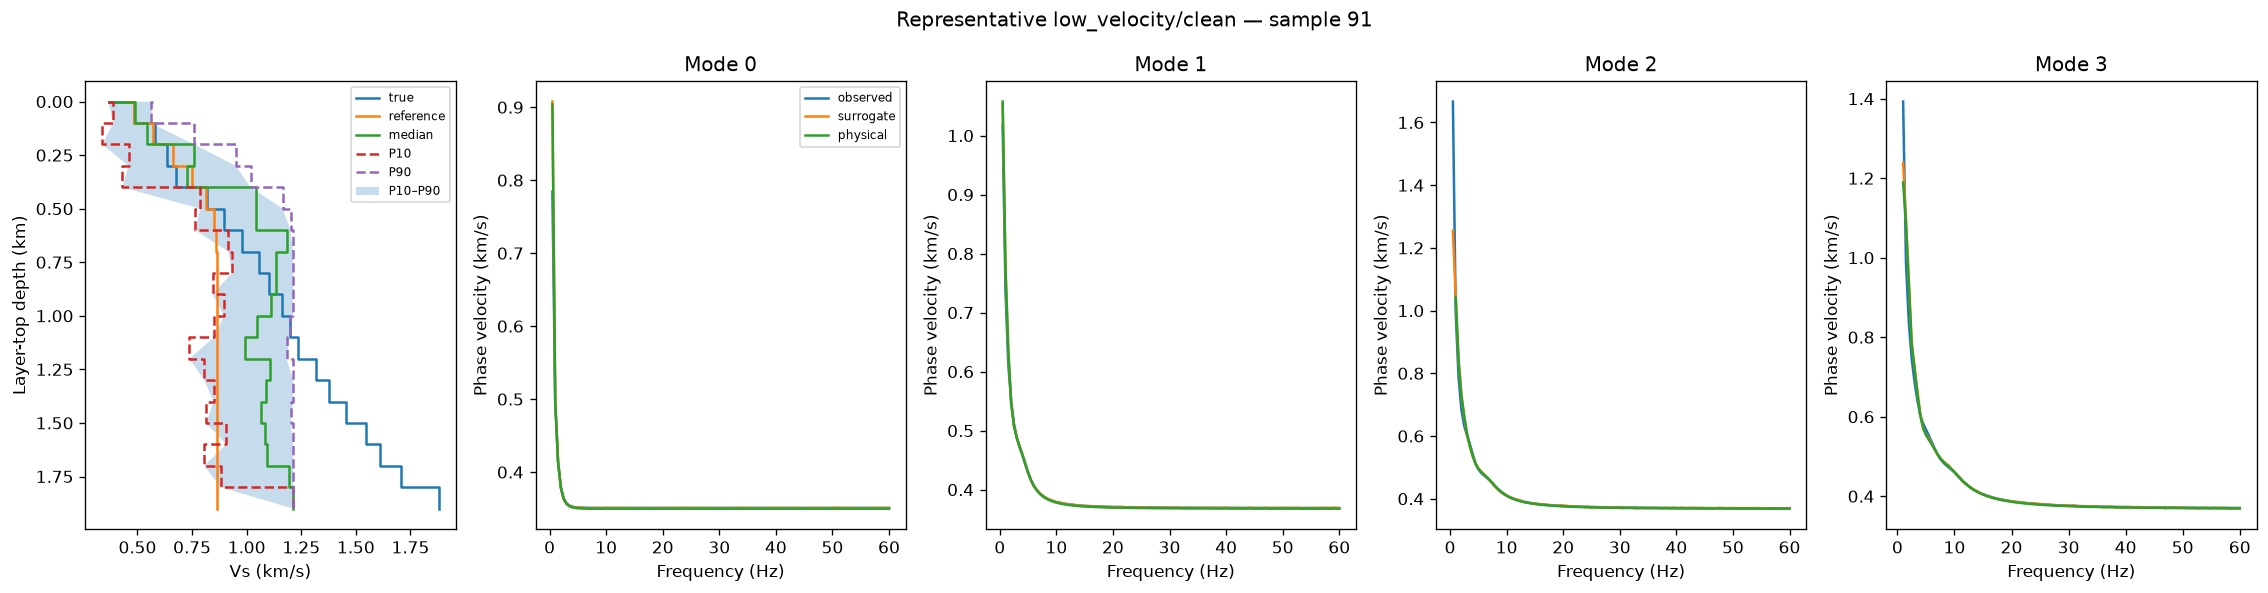
\includegraphics[width=\textwidth]{figures/representative-low_velocity-clean.png}
\caption{代表性低速族样本（clean，样本 91；\texttt{representative-low\_velocity-clean.png}）。
左：真值/参考/中位数/P10/P90 Vs 剖面；右四幅：M0--M3 观测、代理与物理重构曲线。}
\label{fig:rep-lvl}
\end{figure}

\begin{figure}[H]
\centering
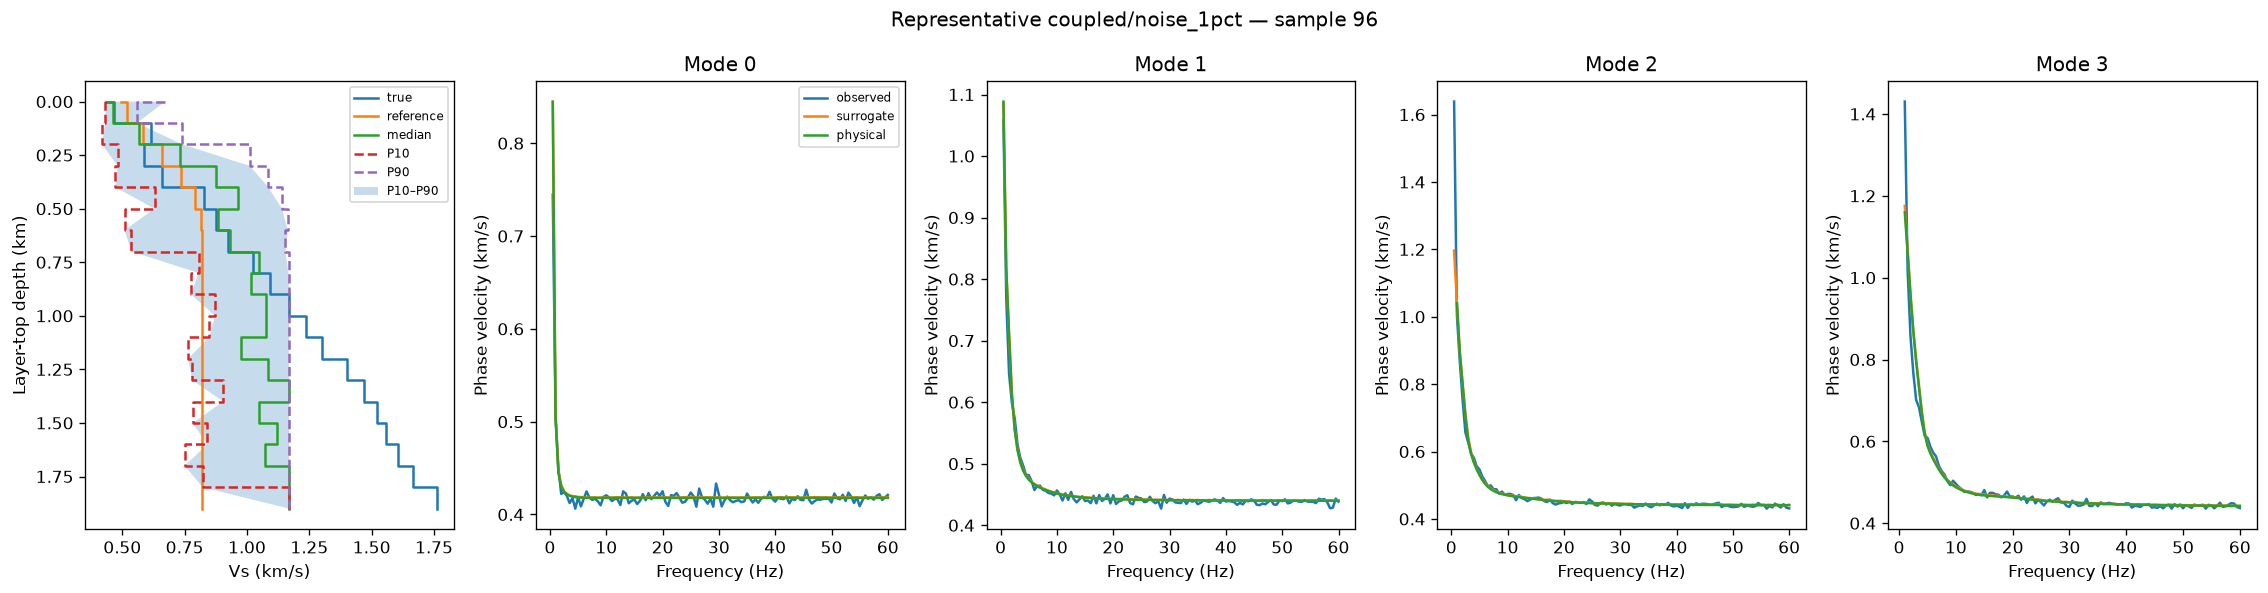
\includegraphics[width=\textwidth]{figures/representative-coupled-noise_1pct.png}
\caption{代表性耦合族样本（noise\_1pct，样本 96；
\texttt{representative-coupled-noise\_1pct.png}）。1\% 噪声下频散重构仍近乎重合，
但深部 Vs 恢复显著失真。}
\label{fig:rep-coupled}
\end{figure}

\section{监督直接反演训练与精度}\label{sec:supervised}
正式运行的 \texttt{run-identity.json} 与 \texttt{evaluation.json} 在数据集
清单 SHA-256、训练样本摘要、模型配置、有序种子集合与划分标识上全部一致。
四折分别含训练 800{,}000、验证 50{,}000、测试 50{,}000 和反演保留 100{,}000 个样本。
训练日志包含 450 条完整轮次记录，三个种子都连续运行
0--149 轮，无缺轮、重复、异常或非有限指标。

\subsection{训练与验证}
三个种子均在训练后期继续改善，因而都达到 150 轮上限而非触发 15 轮早停。最佳轮次与
验证指标见表 \ref{tab:supervised-training}。三种子最佳检查点的等权集成验证 MAE 为
0.026311 km/s，比最佳单种子的 0.027049 km/s 低 2.73\%。

\begin{table}[H]
\centering
\caption{三种子监督反演训练与验证结果（轮次从 0 计数）}
\label{tab:supervised-training}
\begin{tabular}{lccc}
\toprule
种子 & 完成轮数 & 最佳轮次 & 最佳验证 MAE (km/s) \\
\midrule
0 & 150 & 148 & 0.027106 \\
1 & 150 & 149 & 0.027049 \\
2 & 150 & 148 & 0.027062 \\
\midrule
\multicolumn{3}{l}{三种子最佳检查点等权集成} & 0.026311 \\
\bottomrule
\end{tabular}
\end{table}

\subsection{85--89 正式测试折}
三个最佳检查点全部定型后，才对 50{,}000 个测试样本进行一次等权集成评估。总体
MAE 为 0.026291 km/s，RMSE 为 0.049643 km/s，P95 绝对误差为
0.101461 km/s，逐层 \(R^2\) 平均值为 0.9592（表 \ref{tab:supervised-test}）。测试 MAE
与验证集成 MAE 仅差 \(2.0\times10^{-5}\) km/s，未见明显泛化落差。正常族最容易恢复；
高速族 MAE 最高，但四族均保持在 0.031 km/s 以下。

\begin{table}[H]
\centering
\caption{85--89 正式测试折的三种子监督集成 Vs 精度}
\label{tab:supervised-test}
\small
\begin{tabular}{lccccc}
\toprule
族 & 样本数 & MAE (km/s) & RMSE (km/s) & P95 (km/s) & 层平均 \(R^2\) \\
\midrule
normal & 12{,}456 & 0.01867 & 0.03596 & 0.07071 & 0.9791 \\
high\_velocity & 5{,}001 & 0.03037 & 0.05517 & 0.11571 & 0.9472 \\
low\_velocity & 7{,}436 & 0.02964 & 0.05289 & 0.11252 & 0.9522 \\
coupled & 25{,}107 & 0.02827 & 0.05321 & 0.10819 & 0.9550 \\
\midrule
总体 & 50{,}000 & 0.02629 & 0.04964 & 0.10146 & 0.9592 \\
\bottomrule
\end{tabular}
\end{table}

\subsection{90--99 同样本比较}
反演保留折仅在训练、早停和三个最佳检查点全部固定后做一次只读推理，完全不参与模型选择。
这使其可与第 \ref{sec:inversion} 节的 L-BFGS-B clean 在相同 100{,}000 个样本、相同
20 层 Vs 值上直接比较。表 \ref{tab:supervised-comparison} 显示，监督集成 MAE 为
0.026331 km/s，比 L-BFGS-B 的 0.304444 km/s 低 91.35\%（约 11.56 倍）；RMSE
和 P95 绝对误差分别低 88.33\% 和 88.72\%。

\begin{table}[H]
\centering
\caption{90--99 反演保留折上的同样本 Vs 恢复比较（单位均为 km/s）}
\label{tab:supervised-comparison}
\begin{tabular}{lcccc}
\toprule
方法 & 样本数 & MAE & RMSE & P95 绝对误差 \\
\midrule
L-BFGS-B，全量 clean & 100{,}000 & 0.30444 & 0.42543 & 0.89888 \\
三种子监督集成 & 100{,}000 & 0.02633 & 0.04966 & 0.10141 \\
\midrule
监督集成降低比例 & --- & 91.35\% & 88.33\% & 88.72\% \\
\bottomrule
\end{tabular}
\end{table}

改善并非由某一模型族独占：四族 MAE 均下降 88.5\%--93.1\%（表
\ref{tab:supervised-kind-comparison}）。逐层结果更清楚地区分两种方法（图
\ref{fig:supervised-depth-comparison}）：监督集成逐层 MAE 由表层 0.00076 km/s 增至
1.9 km 的 0.04666 km/s，而 L-BFGS-B 在 1.7 km 达 0.77195 km/s；监督集成的逐层最大
绝对偏差仅 0.00131 km/s，未出现 L-BFGS-B 深部接近 \(-0.8\) km/s 的系统性低估。

\begin{table}[H]
\centering
\caption{90--99 同样本比较折按模型族的 Vs MAE（km/s）}
\label{tab:supervised-kind-comparison}
\begin{tabular}{lcccc}
\toprule
族 & 样本数 & L-BFGS-B clean & 监督集成 & 降低比例 \\
\midrule
normal & 25{,}056 & 0.26940 & 0.01861 & 93.1\% \\
high\_velocity & 10{,}074 & 0.26390 & 0.03023 & 88.5\% \\
low\_velocity & 14{,}791 & 0.32227 & 0.02992 & 90.7\% \\
coupled & 50{,}079 & 0.32487 & 0.02835 & 91.3\% \\
\bottomrule
\end{tabular}
\end{table}

\begin{figure}[H]
\centering
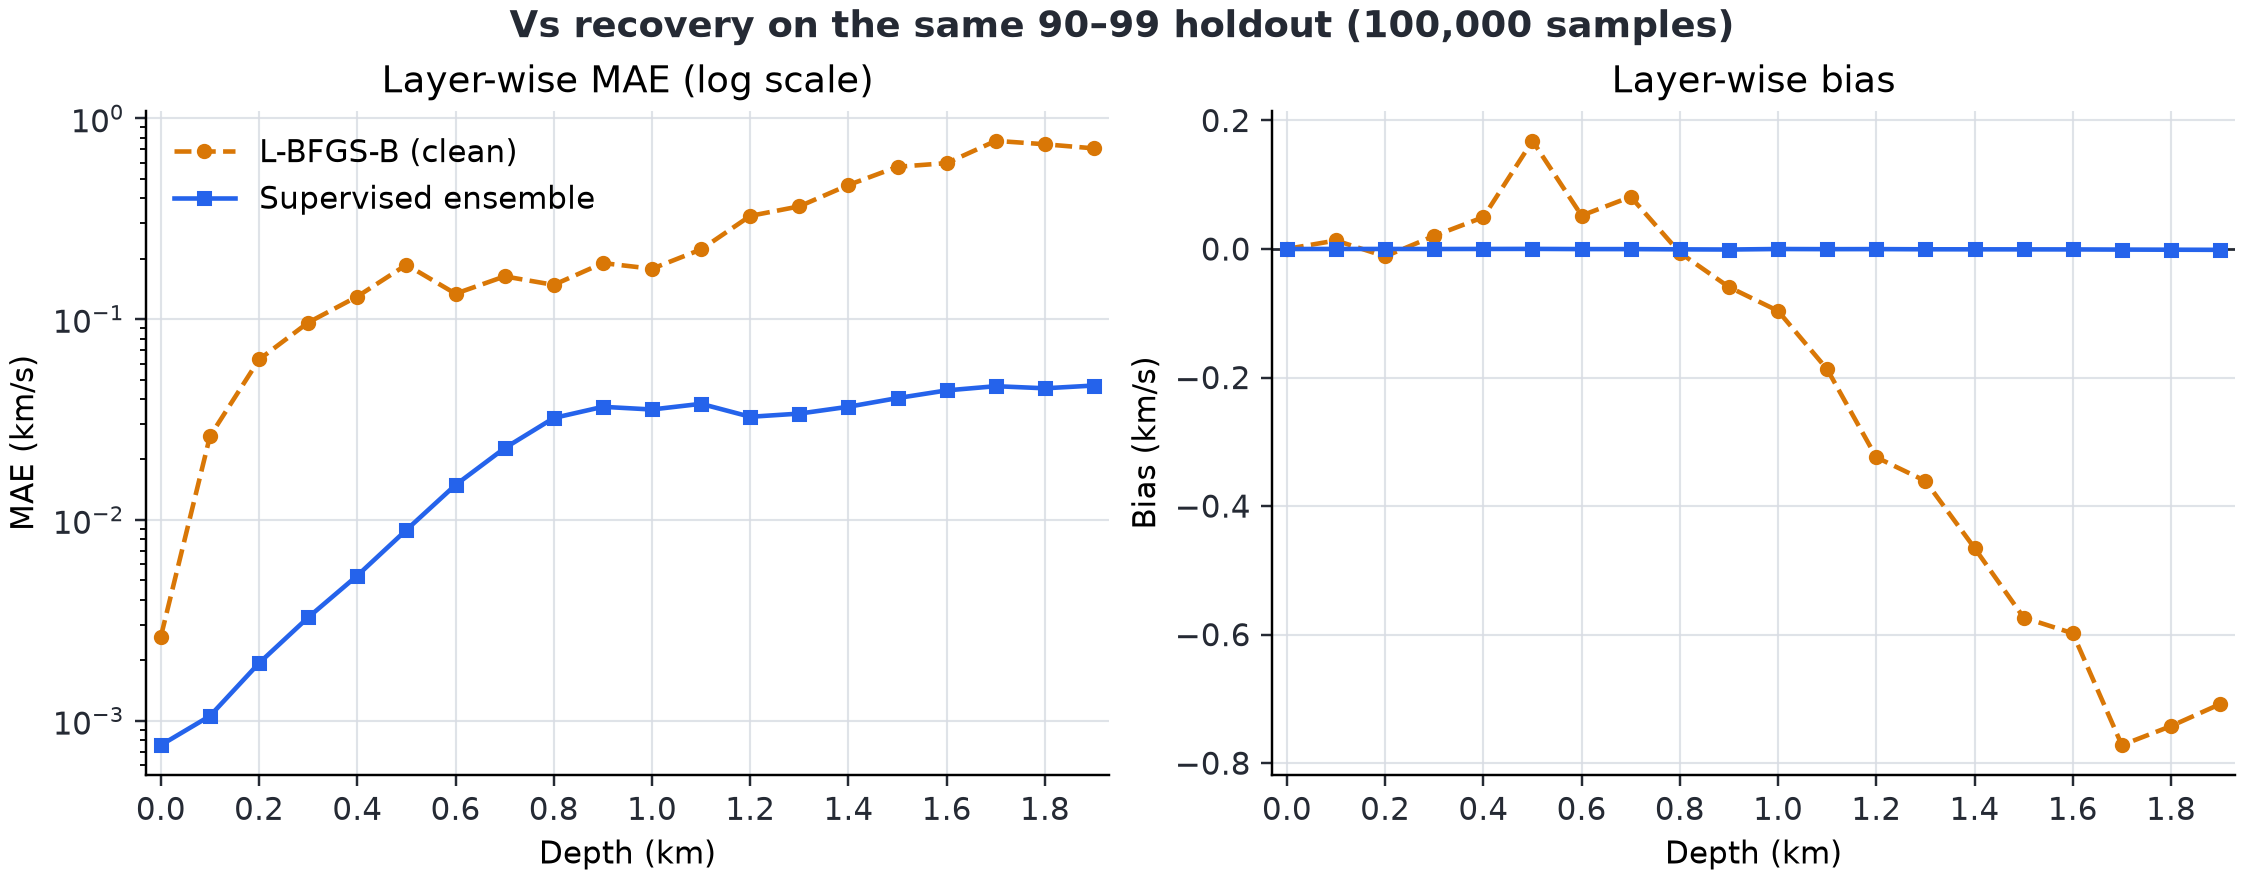
\includegraphics[width=\textwidth]{figures/supervised-vs-lbfgsb-by-depth.png}
\caption{90--99 反演保留折上三种子监督集成与 L-BFGS-B clean 的逐层 Vs 误差。
左图 MAE 使用对数纵轴；右图为有符号偏差。两种方法共享完全相同的 100{,}000 个样本。}
\label{fig:supervised-depth-comparison}
\end{figure}

这是严格同样本、同单位的精度比较，但不是等信息预算的方法学竞赛：监督网络直接使用来自同一合成生成器的
800{,}000 对频散--Vs 标签学习强统计先验；L-BFGS-B 仅在当前参考模型、有界搜索与弱光滑正则下
逐样本拟合观测。因此，结果证明监督先验在当前合成分布内显著更有效，不证明它对未见地质或实测数据
仍保持同等优势；且监督输出本身不提供可校准的不确定性区间。深度多起点结果只有 400 个分层样本，
故仍不与本节的 100{,}000 样本总体值作严格数值对照。

\section{灵敏度加权学习先验的混合反演实验}\label{sec:hybrid}

本节对应第 \ref{sec:hybrid-method} 节的新混合方法。为避免把不同样本折和观测情景混为一谈，
正式主结论统一使用第 90--99 块 \texttt{inversion} 保留折在 \texttt{clean} 情景下的
100{,}000 个唯一模型；同一批模型的 \texttt{noise\_1pct} 只用于稳健性分析。第 85--89 块
\texttt{test} 折仅作为次要复现，不参与主效应数字。两折均完成 200/200 个分片，每个模型均
运行全局边界控制组和混合组，全部准备、控制优化和混合优化的失败数均为零。清单、调参文件和
汇总 JSON 共享数据集、正演检查点、三种子监督检查点、调参文件与源码摘要，且样本 ID 摘要互异，
满足分折隔离。

\subsection{验证集选择的先验强度位于候选上边界}

全局先验系数只用 80--84 验证折按四族各 100 个样本选择，共 400 个唯一模型；每个候选
同时汇总 clean 和 1\% 高斯噪声。表 \ref{tab:hybrid-tuning} 显示验证 MAE 随
\(\lambda_p\) 增大持续下降，配置候选中选择 \(\lambda_p=1.0\)。相对
\(10^{-4}\)，验证 MAE 下降 83.93\%。但最优值落在搜索上边界，因而这里只能解释为
``已测试候选中的最优值''，不能声称已经找到连续参数空间的全局最优点。

\begin{table}[H]
\centering
\caption{学习先验全局系数的验证集选择（400 个唯一模型，两种观测情景合并）。}
\label{tab:hybrid-tuning}
\begin{tabular}{cc}
\toprule
\(\lambda_p\) & 验证 Vs MAE (km/s) \\
\midrule
\(10^{-4}\) & 0.24968 \\
\(10^{-3}\) & 0.23618 \\
\(10^{-2}\) & 0.13102 \\
\(10^{-1}\) & 0.04612 \\
\textbf{1.0} & \textbf{0.04013} \\
\bottomrule
\end{tabular}
\end{table}

\subsection{clean 主比较：混合方法相对全局边界控制组降低 89.34\%}

表 \ref{tab:hybrid-inversion-overall} 给出四种通过精确样本身份门控的方法：旧窄边界
L-BFGS-B、全局边界控制组、灵敏度加权混合反演，以及混合分片中实际保存的三种子监督先验预测。
旧基线的身份由 280 个原始 HDF5 分片只读重建；其 100{,}000 样本摘要与混合反演折完全一致。
在主口径 clean 下，每种方法均评估相同的 200 万个 Vs 单元：MAE 依次为
0.30444、0.25692、0.02739 和 0.02633 km/s。仅放宽边界使控制组相对旧窄边界降低
15.61\%；再加入灵敏度加权学习先验，混合方法相对控制组降低 89.34\%，相对旧基线降低
91.00\%。混合 MAE 比直接监督预测高 4.04\%，说明 \(\lambda_p=1\) 时最终解主要由
学习先验决定，而物理目标承担局部校正作用。

\begin{table}[H]
\centering
\caption{90--99 反演保留折的严格同样本总体 Vs 指标；clean 为主比较，noise\_1pct 为稳健性比较；每行 100{,}000 个模型。}
\label{tab:hybrid-inversion-overall}
\small
\begin{tabular}{llrrrr}
\toprule
情景 & 方法 & MAE & RMSE & P95 绝对误差 & 偏差 \\
\midrule
\multirow{4}{*}{clean}
 & 旧窄边界 L-BFGS-B & 0.30444 & 0.42543 & 0.89888 & -0.22598 \\
 & 全局边界控制组 & 0.25692 & 0.35979 & 0.75683 & -0.16088 \\
 & 灵敏度加权混合 & 0.02739 & 0.04991 & 0.10185 & -0.00052 \\
 & 三种子监督先验 & 0.02633 & 0.04966 & 0.10141 & -0.00037 \\
\midrule
\multirow{4}{*}{noise\_1pct}
 & 旧窄边界 L-BFGS-B & 0.30501 & 0.42603 & 0.90003 & -0.22642 \\
 & 全局边界控制组 & 0.25702 & 0.35985 & 0.75675 & -0.16057 \\
 & 灵敏度加权混合 & 0.05491 & 0.08831 & 0.18881 & 0.00007 \\
 & 三种子监督先验 & 0.05469 & 0.08856 & 0.18961 & 0.00044 \\
\bottomrule
\end{tabular}
\end{table}

\subsection{1\% 高斯噪声稳健性：学习型方法误差约翻倍}

在完全相同的 100{,}000 个模型上加入 1\% 高斯噪声后，旧窄边界、全局边界控制、混合和
直接监督的 MAE 分别为 0.30501、0.25702、0.05491 和 0.05469 km/s。混合方法仍比全局边界
控制组低 78.64\%，比旧窄边界低 82.00\%；但相对自身 clean 结果增加 100.45\%，直接监督
也增加 107.69\%。相反，控制组仅增加 0.00010 km/s。这说明强学习先验明显改善恢复精度，
同时会把输入扰动经监督预测传入最终模型。本次协议没有人工随机删除原有效频散单元，因此不能
把该结果解释为对随机缺失的验证。

\subsection{clean 情景的分族与逐层诊断}

这一改善在四种模型族上均存在。表 \ref{tab:hybrid-kind} 只使用主口径 clean：混合方法相对
控制组的 MAE 降低比例为 86.59\%--91.62\%，不是由某一族独占。高速族的改善最小；四族中
混合 MAE 均略高于直接监督先验，说明物理项在当前权重下没有进一步降低总体 Vs 误差。

\begin{table}[H]
\centering
\caption{90--99 反演折 clean 情景按模型族的 Vs MAE。}
\label{tab:hybrid-kind}
\small
\begin{tabular}{lrrrr}
\toprule
模型族 & 全局边界控制组 & 混合反演 & 监督先验 & 混合相对控制降低 \\
\midrule
normal         & 0.23498 & 0.01969 & 0.01861 & 91.62\% \\
high\_velocity & 0.23164 & 0.03105 & 0.03023 & 86.59\% \\
low\_velocity  & 0.26229 & 0.03119 & 0.02992 & 88.11\% \\
coupled        & 0.27139 & 0.02939 & 0.02835 & 89.17\% \\
\bottomrule
\end{tabular}
\end{table}

图 \ref{fig:hybrid-depth} 展示 clean 情景的逐层误差。1.2--1.9 km 八层的平均 MAE 从控制组
0.45658 km/s 降至混合组 0.04065 km/s，与监督先验的 0.04072 km/s 基本相同；混合方法
消除了控制组随深度增大的系统性失真。在最浅的 0.1--0.3 km，混合结果与监督先验的差距
更明显，反映这些较敏感层被允许更多服从物理数据项；在 1.9 km 半空间，混合 MAE
0.04537 km/s 略低于监督先验的 0.04666 km/s。

\begin{figure}[H]
\centering
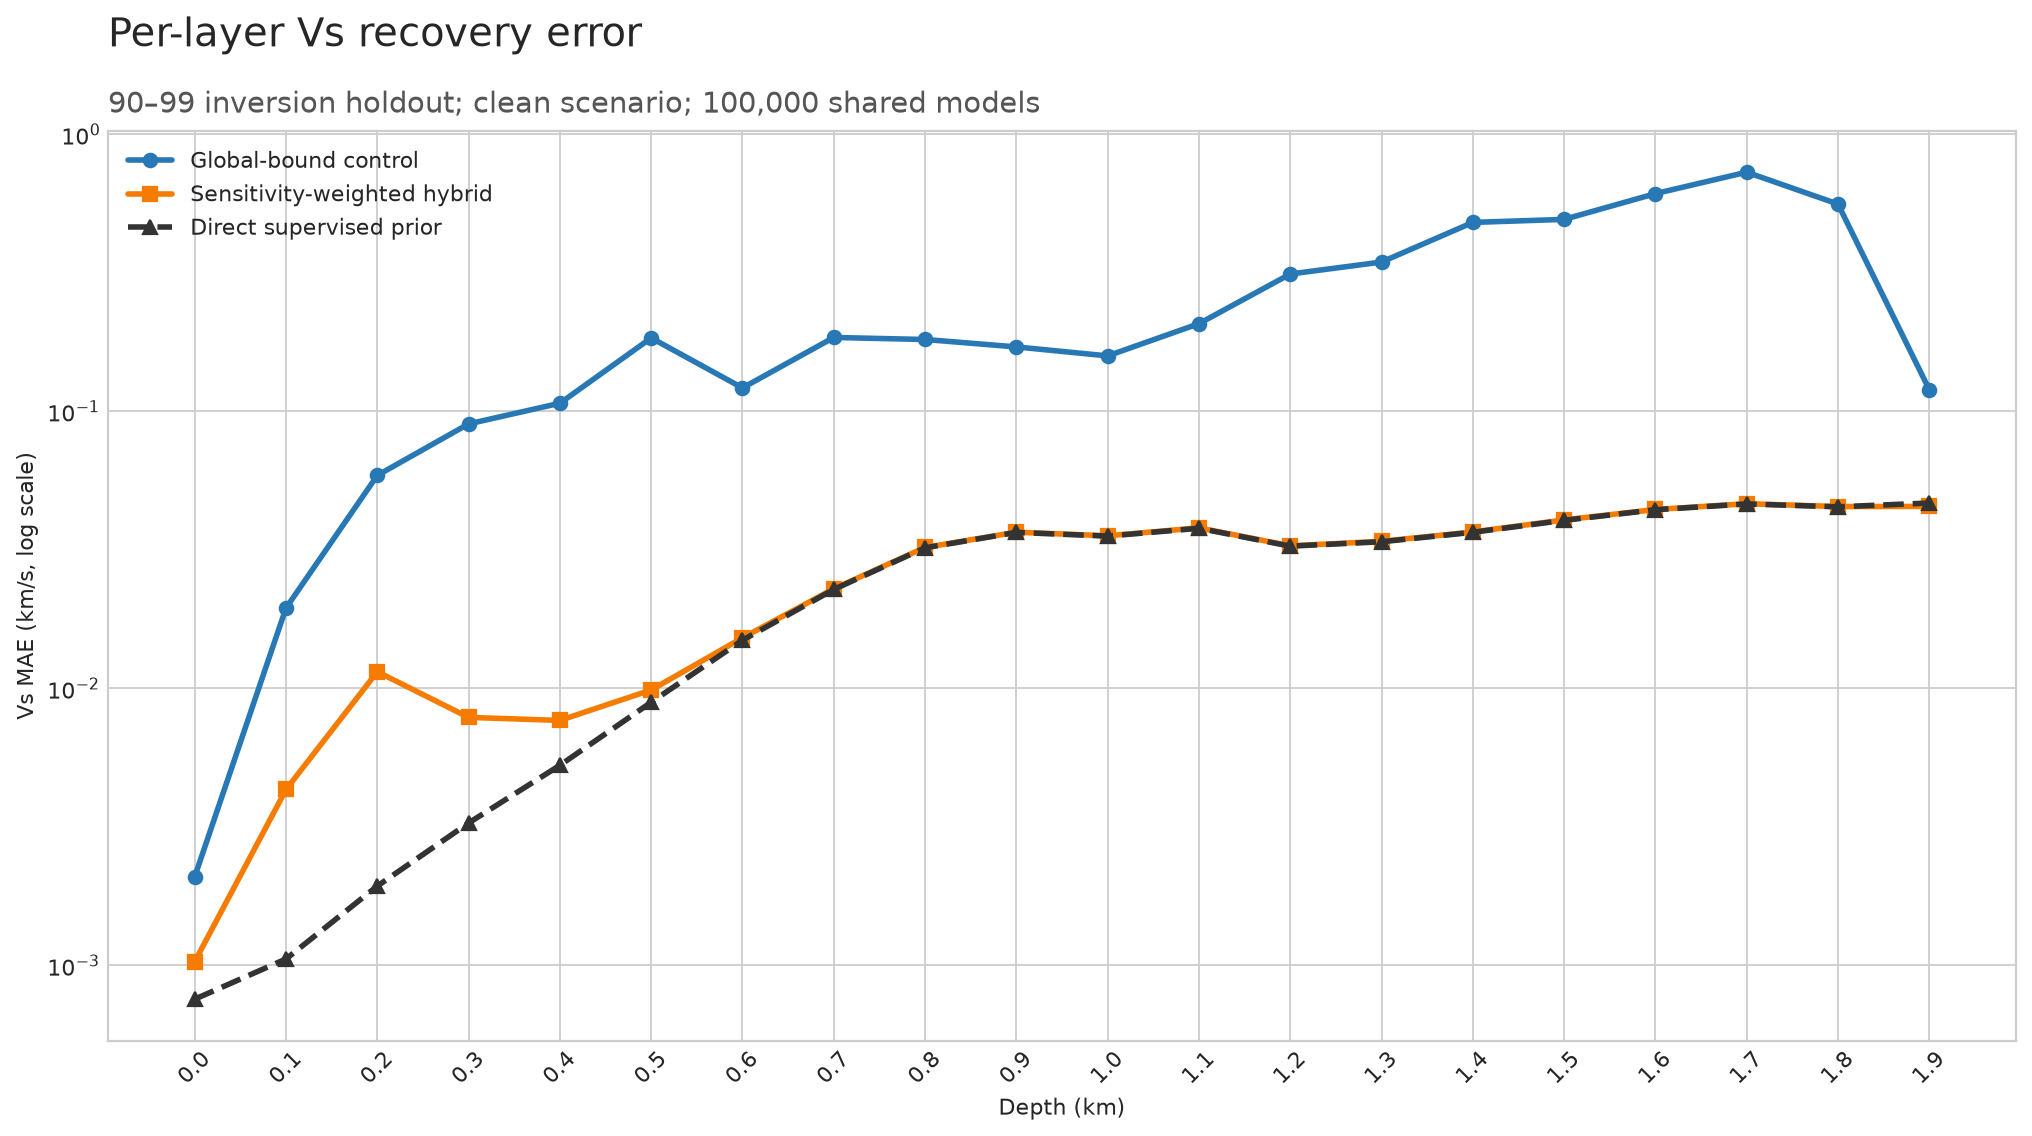
\includegraphics[width=0.98\textwidth]{figures/hybrid-vs-mae-by-depth.png}
\caption{90--99 反演折 clean 情景逐层 Vs MAE（纵轴为对数尺度）。
三条曲线共享相同的 100{,}000 个唯一模型和 20 层真值。}
\label{fig:hybrid-depth}
\end{figure}

\subsection{灵敏度权重符合预期，并降低优化代价}

图 \ref{fig:hybrid-sensitivity} 给出反演折 clean 情景的逐层均值。第 0 层平均无量纲
灵敏度最高（0.90731），对应平均先验权重最低（0.25011）；灵敏度在 1.0 km 达到最低
0.002157，对应权重 1.74674。20 层平均权重严格为 1。由于先对每个样本做逆灵敏度、
截断和均值归一化，再跨样本求均值，``平均灵敏度的倒数''与``平均权重''不要求在所有深层
严格单调对应。

\begin{figure}[H]
\centering
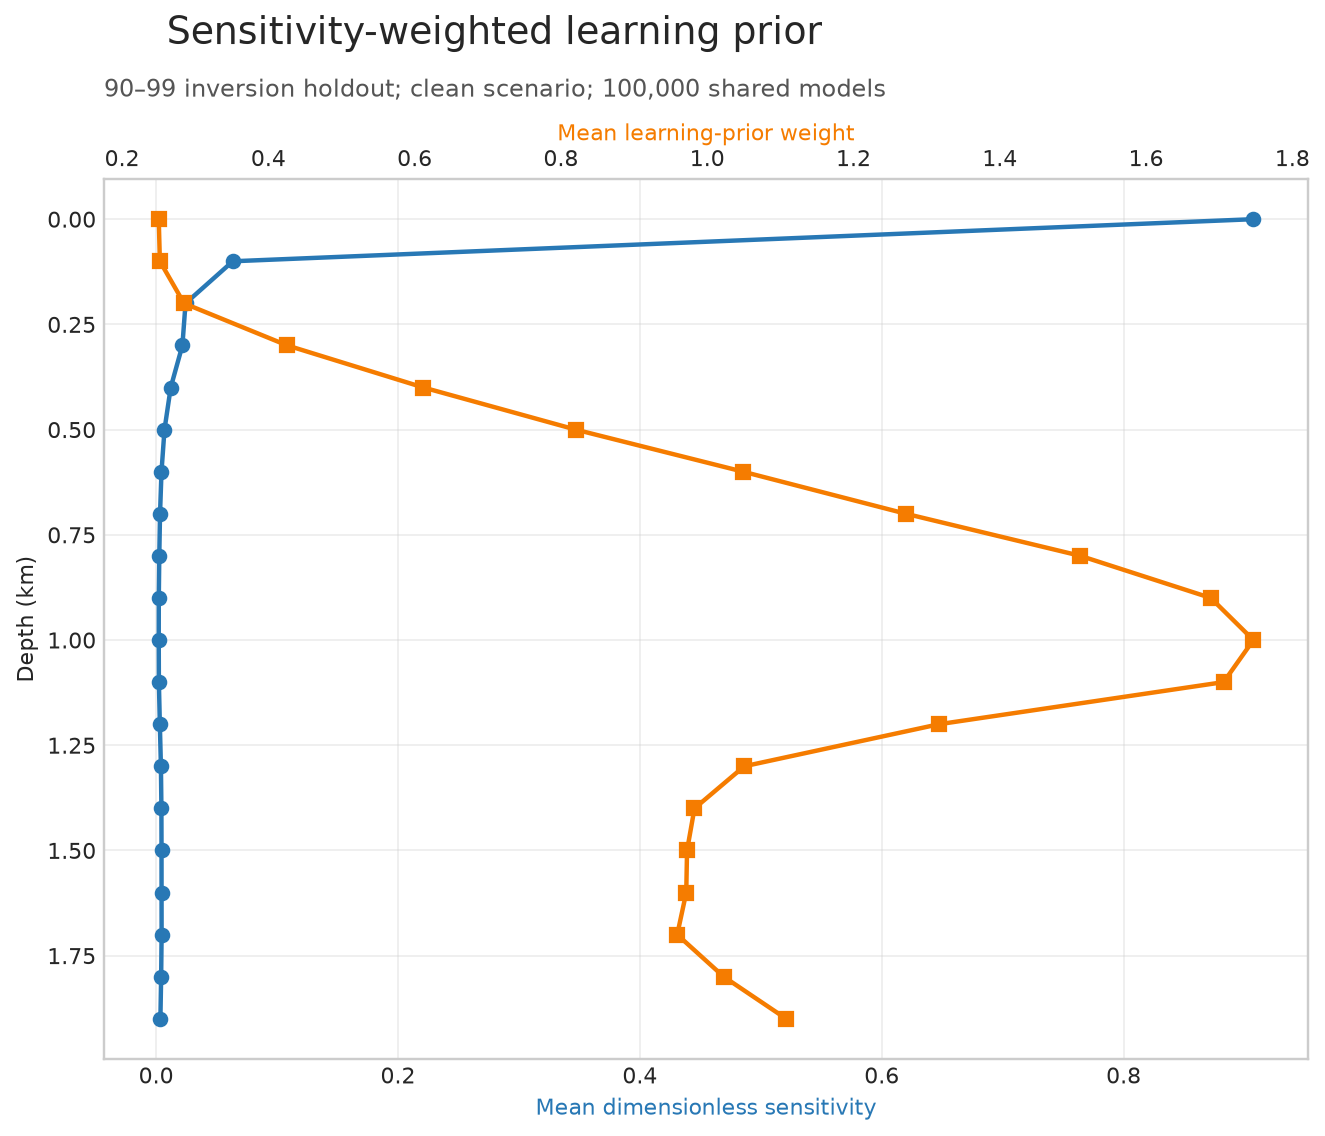
\includegraphics[width=0.88\textwidth]{figures/hybrid-sensitivity-and-prior-weight-by-depth.png}
\caption{90--99 反演折逐层平均无量纲灵敏度（蓝色、下横轴）与学习先验权重
（橙色、上横轴）；仅使用 clean 主口径。低灵敏度层总体获得更强先验约束。}
\label{fig:hybrid-sensitivity}
\end{figure}

表 \ref{tab:hybrid-cost} 显示，学习先验不仅改善 Vs，还缩短了搜索。主口径 clean 下，平均
迭代数从 24.84 降至 17.66（按未舍入均值计算减少 28.89\%），函数求值从 30.84 降至 20.82（减少
32.49\%），代理频散重构 MAE 从 0.00308 降至 0.00092 km/s。1\% 高斯噪声下，迭代数
从 24.85 降至 18.07，函数求值从 30.85 降至 21.26；两种情景的方向一致，但不再把它们
合并成第三套结论数字。

\begin{table}[H]
\centering
\caption{90--99 反演折的优化代价与代理频散重构误差。}
\label{tab:hybrid-cost}
\small
\begin{tabular}{llrrr}
\toprule
情景 & 方法 & 平均迭代数 & 平均函数求值 & 频散重构 MAE \\
\midrule
\multirow{2}{*}{clean}
 & 全局边界控制组 & 24.84 & 30.84 & 0.00308 \\
 & 灵敏度加权混合 & 17.66 & 20.82 & 0.00092 \\
\midrule
\multirow{2}{*}{noise\_1pct}
 & 全局边界控制组 & 24.85 & 30.85 & 0.00591 \\
 & 灵敏度加权混合 & 18.07 & 21.26 & 0.00452 \\
\bottomrule
\end{tabular}
\end{table}

\subsection{复现实验与限制}

85--89 测试折在本次生产运行中只作为次要复现折；它保持与 90--99 主反演折相同的方法排序，
支持同源合成分布内的稳定性，但其指标不再与主结果并排陈述。最终科学结论只使用从训练、调参和
监督测试中隔离的 90--99 反演折；完整测试折数值保留在机器可读汇总 JSON 中。

旧窄边界基线最初的汇总文件没有保存严格门控要求的样本 ID 摘要。现已在不修改原始数据的
前提下，对 280 个 HDF5 分片、清单、文件 SHA、内容 SHA、任务身份和样本身份逐项校验，
重建出 100{,}000 样本摘要；其摘要与混合反演折一致，报告器将基线标记为
\texttt{available}。归档模式只豁免``结果源码摘要等于当前报告器源码摘要''这一项，并在
汇总中同时保留两份源码摘要，其他身份门控不变。外部监督 \texttt{evaluation.json} 仍缺少
精确监督检查点身份，因此正式四方法表中的监督值继续取自混合分片内绑定三份检查点摘要的
监督先验预测。未来仍需补齐外部监督身份，并把 \(\lambda_p>1\) 及随机缺失情景纳入预注册
候选后重新报告。

\section{讨论}\label{sec:discussion}

\paragraph{拟合--恢复分离：非唯一性是弱先验优化的主要误差源}
原始窄边界反演在所有 20.08 万行上 100\% 收敛且频散重构 MAE 达 \(10^{-3}\) km/s 量级。
自然族比例的 10 万模型全量实验总体 Vs MAE 为 0.3047 km/s；四族等量的 400 模型深度实验
绝对 MAE 为 0.2713 km/s，但二者不是同人口对照，不能估计多起点增益。这些结果表明当前
目标函数的极小值域包含大量与真值差异巨大
的等效模型：观测（4 模式 \(\times\) 120 频点）不足以在 20 维模型空间内唯一确定
深部结构。1\% 噪声几乎不改变原始窄边界和新全局边界控制组的恢复精度，进一步证实这两种
弱先验优化的误差预算由结构性非唯一性与先验约束主导，而非数据质量；这一判断不能外推到
监督先验和混合方法，因为二者在相同噪声下的 MAE 均约翻倍。

\paragraph{边界约束的系统性偏差}
逐层边界取自基阶经验深度式构造的参考模型（\(\pm0.35\) km/s）。浅部该近似有效
（第 0 层 MAE 仅 0.003 km/s），但深部灵敏度低、经验深度式失真，真实半空间速度常
落于界外，造成 1.1 km 以下单调增长的负偏差（最大 \(-0.772\) km/s）与区间零覆盖。
这是本管线当前最明确的可改进点：放宽深部边界、引入多参考模型或对边界本身做
分层标定，都可能显著降低深部误差。

\paragraph{不确定性量化不可用}
P10--P90 经验区间总体覆盖率 49.7\%（名义 80\%）且深部为零，表明``同一搜索盒内
多起点的散布''不能刻画真实后验不确定性。任何下游应用不应直接使用该区间。

\paragraph{代理精度的双重角色}
深度子集上，恢复模型相对观测的代理残差为 0.0155 km/s，物理重算残差为 0.0116 km/s；
由于两者有效单元不完全相同，且未直接计算代理--物理预测差，这一结果只说明拟合评价依赖
所用算子，不能量化代理外推误差。独立测试折的总体 MAE 为
\(1.80\times10^{-4}\) km/s，表明代理在数据生成分布内精度很高；但反演优化会主动
搜索偏离训练分布的速度模型，因此分布内测试精度不能保证优化路径上的局部代理精度。
后续应在共同有效单元上直接报告代理与物理预测的差异；在此之前，物理重校验仍不可省略。

\paragraph{混合实验确认学习型先验是主要改善来源}
优化反演的目标只含数据拟合与弱光滑先验，会在非唯一方向上自由移动；监督网络则从 80 万标签样本学得
深部高速半空间、背景速度趋势和异常族的联合统计先验。同样本 MAE 低 91.35\% 且深部偏差几乎消失，
支持“先验与搜索边界是当前 L-BFGS-B 重要短板”的解释，而不支持将误差归因于目标函数未收敛。
新的配对控制进一步分离了两种作用：在 clean 主口径下，仅把边界放宽到全局范围，MAE 从
0.30444 降至 0.25692 km/s；加入灵敏度加权学习先验后降至 0.02739 km/s，且深层平均误差
降低近一个数量级。混合结果比直接监督预测的 0.02633 km/s 高 4.04\%，说明当前最优候选下的
增益主要来自监督统计先验，而不是物理项独立恢复了
同等结构。但是，这一优势只在与训练集同源的合成测试与保留折上获得验证；分布外地质、不同层厚、
随机缺失、实测噪声与模态误标都可能缩小该差距。监督点预测也未给出可校准的不确定性，不应将本结果
外推为对实测反演的普遍优越性证明。

\paragraph{噪声稳健性与系数选择仍不充分}
控制组对 1\% 高斯噪声近乎不敏感，但混合与监督方法的 MAE 分别增加 100.45\% 和 107.69\%，
显示强学习先验把输入扰动通过监督预测传入最终模型。另一方面，验证 MAE 在候选范围内随
\(\lambda_p\) 单调下降且最优值为上界 1.0，尚不能排除更强先验继续改善或开始过拟合的可能。
后续稳健性实验应预先固定更宽的对数候选网格，并加入确定性随机缺失，而不是在看到当前结果后
选择性扩展单一情景。

\paragraph{工程完整性}
结果模式 v3 与混合结果模式分别将数据集清单、检查点、配置、源码摘要与精确样本身份绑定；分片原子发布、
断点恢复与任务模划分均经损坏/恢复类测试验证。新增审计器进一步验证百万样本身份、
跨折精确重复和逐样本地质重建；监督训练器的恢复会拒绝数据、划分、种子集合、模型或训练配置
不一致的检查点，并以最后发布的 \texttt{last.pt} 作为轮次提交记录。混合实验两折各 200 个
作业全部完成，且把控制与混合失败状态独立保存。严格门控先暴露了旧基线汇总缺少样本身份，
随后通过只读原始分片迁移闭合该缺口；外部监督检查点身份缺口仍被明确保留，避免用不可审计的
外部值替换分片内已绑定的监督预测。完整测试与静态检查结果列于附录
\ref{app:repro}。

\section{结论}\label{sec:conclusion}
本项目交付了从确定性数据生成、物理正演、神经代理到可审计反演实验的完整管线，
并完成了百万样本数据集、300 轮代理训练、旧窄边界在 clean 与 1\% 高斯噪声下各 10 万行的
反演、8 万起点的深度多起点
实验、三种子各 150 轮的监督直接反演，以及验证调参加 test/inversion 两折的混合反演生产实验。
结果均有据可查：正演与代理环节精度优异（验证 MAE
\(1.82\times10^{-4}\) km/s，独立测试 MAE \(1.80\times10^{-4}\) km/s），百万样本
审计未发现地质规则违规、精确重复或跨折重复；反演环节则暴露了非唯一性主导的本质困难——
很小的频散残差并未转化为可用的 Vs 恢复：全量自然族比例实验 MAE 为 0.3047 km/s，
四族等量深度实验的绝对 MAE 为 0.2713 km/s，但二者不能用于估计多起点增益；经验不确定性
区间严重欠覆盖（49.7\%），深部存在边界约束导致的系统性负偏差。监督集成则在独立测试折取得
0.02629 km/s MAE。统一到 90--99 同样本、clean 主口径后，旧窄边界、全局边界控制、混合反演和
直接监督的 MAE 依次为 0.30444、0.25692、0.02739 和 0.02633 km/s；混合方法相对全局边界
控制组降低 89.34\%，平均迭代数降低 28.89\%，深层 1.2--1.9 km 平均 MAE 从 0.45658 降至
0.04065 km/s。1\% 高斯噪声作为独立稳健性结果，使混合 MAE 增至 0.05491 km/s，但仍比同情景
控制组低 78.64\%。该结果说明学习型先验能有效解除当前合成分布内的深部欠约束；但验证最优
系数落在候选上边界，且噪声使学习型方法误差约翻倍，尚不构成实测地质上的外部验证。后续工作的优先级：
（1）预注册并验证 \(\lambda_p>1\) 的候选；（2）增加随机缺失、模态误标和分布外地质；
（3）补齐外部监督评估的精确检查点身份元数据；（4）为监督预测增加可校准的不确定性，
并保留物理重校验作为反演成功判据的可选路径。

\appendix
\section{可核验性、归档边界与产物清单}\label{app:repro}
\begin{sloppypar}
当前 Git 交付支持对汇总数字、身份摘要和报告推导的只读核验，但不支持从原始数据重新训练、
反演或生成全部汇总。以下清单明确区分``已版本化''、``可由汇总核验''和``原始产物缺失''，
避免把摘要级审计误写成端到端复现。

\begin{itemize}
\item \textbf{已版本化的代码与报告：}源代码和生产配置位于 \texttt{src/} 与
      \texttt{configs/}；正式报告源码、PDF、所引用图片和小型证据位于
      \texttt{docs/final-report/}。报告目录中的 \texttt{README.md} 给出编译方式与归档边界。
\item \textbf{已版本化的旧反演汇总：}
      \texttt{results/inversion-report/summary.json} 与 11 幅报告图；结果身份绑定数据集清单
      \texttt{ceecda31ae9dec3f\ldots}、正演检查点 \texttt{b1a6fc08a40ba648\ldots}、
      源码 \texttt{06f66599106b57f2\ldots} 和划分
      \texttt{mod100-v2-80-5-5-10}。
\item \textbf{已版本化的监督元数据：}
      \texttt{runs/supervised-inversion-v2/} 保存 \texttt{run-identity.json}、三份
      \texttt{seed-*-history.json}、\texttt{training.log} 与 \texttt{evaluation.json}；
      评估 JSON SHA-256 为 \texttt{155cf66eda488a5d\ldots}。这些文件不含模型权重。
\item \textbf{已版本化的混合汇总：}
      \texttt{results/hybrid-inversion/tuning.json}、test/inversion 两份清单和
      \texttt{results/hybrid-inversion-report/summary.json}。清单各记录 200/200 作业完成；
      汇总绑定源码 \texttt{6eb0857f02b81071\ldots}、三份监督检查点摘要
      \texttt{cb8aa290\ldots}/\texttt{dc0cd1f\ldots}/\texttt{ea17d288\ldots}，并记录
      400 个调参样本与 \(\lambda_p=1.0\)。
\item \textbf{汇总级可核验范围：}现有 JSON 足以复核本报告的总体、分族、逐层指标、候选
      \(\lambda_p\)、样本人口摘要和正文百分比。旧窄边界人口摘要
      \texttt{fbedb8df6accf778\ldots} 与混合反演折一致，外部基线状态为
      \texttt{available}；这证明已归档汇总之间身份一致，不等于原始字节仍可取得。
\item \textbf{当前 Git 缺失的原始产物：}\texttt{data/production} 的 100 个数据分片及清单、
      \texttt{runs/production-48g} 的正演检查点与训练产物、
      \texttt{results/inversion} 的 280 个原始 HDF5 分片、混合反演原始 HDF5 分片，以及
      三个监督 \texttt{seed-*-best.pt} 均不在当前检出中。生产数据生成与正演训练的主机墙钟
      耗时也未归档。
\item \textbf{缺失造成的限制：}当前检出不能重新执行百万样本审计、训练模型、重跑反演、
      从原始分片再次生成报告，也不能补算同 400 样本的单起点对照或代理--物理直接差异。
      摘要中保存的 SHA-256 可验证身份记录，但不能代替缺失的原始字节。
\item \textbf{小型证据：}\texttt{docs/final-report/evidence/} 保存数据审计 JSON、正演测试
      JSON 和监督比较绘图脚本；它们支持报告中的对应汇总声明，但不能替代数据集与检查点。
\item \textbf{当前可运行检查：}\texttt{python -m pytest -q} 与
      \texttt{ruff check src tests scripts} 验证代码；在 \texttt{docs/final-report/} 内运行
      \texttt{tectonic -X compile report.tex} 可重编本报告。2026-08-17 本机复核为
      307 passed，Ruff 全部通过。
\item \textbf{条件式重建命令：}只有先从独立生产归档恢复上述数据、检查点与 HDF5 分片后，
      才能运行 \texttt{swave inversion-report} 或 \texttt{swave hybrid-report} 重新生成汇总；
      当前报告不把这两个命令列为可直接执行的复现步骤。
\item \textbf{外部监督身份限制：}外部 \texttt{evaluation.json} 缺少精确检查点摘要；正式
      四方法比较使用混合分片内绑定三份检查点摘要的监督预测。外部评估仍只作为训练与测试元数据证据。
\end{itemize}
\end{sloppypar}

\begin{thebibliography}{9}
\bibitem{pan-mode-kissing}
Lei Pan and Xiaofei Chen,
\emph{Efficient Computation of Dispersion Curves in Low-Velocity-Layered Half-Spaces},
投稿稿 \texttt{bssa-2025003.1.pdf}；参考代码：
\url{https://github.com/pan3rock/mode-kissing}。

\bibitem{pan-qedispinv}
Lei Pan, Jiannan Wang and Xiaofei Chen,
\emph{Surface-Wave Dispersion Curve Computation and Inversion},
投稿稿 \texttt{bssa-2025207.1.pdf}；参考代码：
\url{https://github.com/pan3rock/QEDispInv}。
\end{thebibliography}

\end{document}
